%%%%%%%%%%%%%%%%%%%%%%%%%%%%%%%%%%%%%%%%%
% fphw Assignment
% LaTeX Template
% Version 1.0 (27/04/2019)
%
% This template originates from:
% https://www.LaTeXTemplates.com
%
% Authors:
% Class by Felipe Portales-Oliva (f.portales.oliva@gmail.com) with template 
% content and modifications by Vel (vel@LaTeXTemplates.com)
%
% Template (this file) License:
% CC BY-NC-SA 3.0 (http://creativecommons.org/licenses/by-nc-sa/3.0/)
%
%%%%%%%%%%%%%%%%%%%%%%%%%%%%%%%%%%%%%%%%%

%----------------------------------------------------------------------------------------
%	PACKAGES AND OTHER DOCUMENT CONFIGURATIONS
%----------------------------------------------------------------------------------------

\documentclass[
	12pt, % Default font size, values between 10pt-12pt are allowed
	%letterpaper, % Uncomment for US letter paper size
	%spanish, % Uncomment for Spanish
]{fphw}

% Template-specific packages
\usepackage[utf8]{inputenc} % Required for inputting international characters
\usepackage[T1]{fontenc} % Output font encoding for international characters
\usepackage{mathpazo} % Use the Palatino font

\usepackage{graphicx} % Required for including images

\usepackage{booktabs} % Required for better horizontal rules in tables

\usepackage{listings} % Required for insertion of code

\usepackage{enumerate} % To modify the enumerate environment

%----------------------------------------------------------------------------------------
%	ASSIGNMENT INFORMATION
%----------------------------------------------------------------------------------------

\title{Introducción a Heroku} % Assignment title

\author{Michael Jefferson Ballesteros Coca} % Student name

\date{Agosto 20, 2020} % Due date

\institute{Escuela Colombiana de Ingeniería Julio Garavito \\ Decanatura Ingeniería de Sistemas} % Institute or school name

\class{Arquitecturas Empresariales} % Course or class name

\professor{Luis Daniel Benavides Navarro} % Professor or teacher in charge of the assignment

%----------------------------------------------------------------------------------------

\begin{document}

\maketitle % Output the assignment title, created automatically using the information in the custom commands above

%----------------------------------------------------------------------------------------
%	ASSIGNMENT CONTENT
%----------------------------------------------------------------------------------------


\subsection * {Program Requirements}

\begin {enumerate} [(a \normalfont)]% Sub-questions styled as italic letters
\item The program reads n real numbers from a web page
\item Test the program with tables 1 and 2
\item Use a LinkedList to store the n numbers for calculations.
\end {enumerate}
% ------------------------------------------------

\subsection * {General}

\subsection * {LinkedList}

LinkedLists are common data structures where data is stored, they are implemented with pointers, which allow the data that is used to be chained from memory addresses.
LinkedLists have 2 main components:
\begin {itemize}
\item List head
\item Nodes
\end {itemize}

There are several options to create this structure, for this repository, the LinkedList has a head, where it has 2 pointers, one towards the beginning of the LinkedList and another towards the last node of the structure.

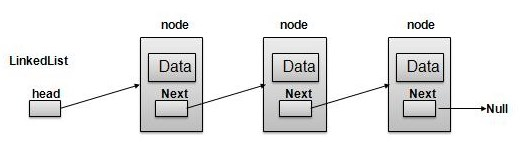
\includegraphics [scale = 0.8] {OgP3r.jpg}

It also has different functionalities that were implemented, among them:

\begin {itemize}
\item add ()
\item remove ()
\item size ()
\item toArray ()
\end {itemize}
% ------------------------------------------------- ---------------------------------------


% ------------------------------------------------

\subsection * {Media}



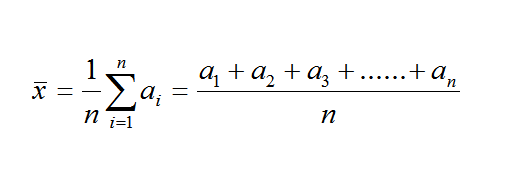
\includegraphics [scale = 0.8] {formula-media.png}


When we look for the mean of a set of data, we locate the position of the center of these through the average of these.

The Calculator class in the repository has a method (calculateMean ())

\begin{verbatim}
public static Double calculateMean (Double [] array) {
        Double sum = 0d;
        int n = array.length;
        for (Double x: array) {
            sum + = x;
        }
        return sum / n;
    }
\end{verbatim}

Where, a For loop was used to traverse the data and a variable (sum) is carried to perform the sum of the data; It is concluded after going through the data, the mean, calculating with the value n the amount of data that exist and the sum of all the data.

% ------------------------------------------------- ---------------------------------------
\subsection * {Standard Deviation}

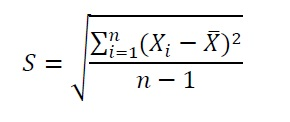
\includegraphics [scale = 0.8] {2583684_orig.jpg}

The standard deviation quantifies the variation of the population, although it would appear more robust with respect to the average if calculated with pencil and paper, it could be a complex procedure.

A method was implemented in the Calculator class to calculate the standard deviation (calculateDeviation ())

\begin{verbatim}
public static Double calculateDeviation (Double [] array, double mean) {
        Double sumx = 0d;
        int n = array.length;
        for (Double x: array) {
            sumax + = Math.pow (x-mean, 2);
        }
        return Math.sqrt ((sumx / (n-1)));
    }
\end{verbatim}

This time, we use the For loop to determine the internal part of the root, where a variable (sumax) was carried where the calculation was made between the average and each piece of data in the data set. The method ends by returning the square root of the inner part of the root, using the Java Math library.


% ------------------------------------------------

\subsection * {Absolute Error}

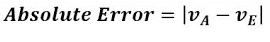
\includegraphics [scale = 0.8] {Capture.JPG}


In order to check our calculations, we need to use the absolute error and have a tolerance margin, since with this we can tell if the resulting data is reliable or not.

\begin{verbatim}
private static Double TOLERANCE = 0.1d;

@Test
public void shouldCalculateMean () {
    String file = "src \\ test \\ resources \\ data \\ data1.txt";
    LinkedList list = new LinkedList ();
    Calculator.readFile (file, list);
    Double errorAbsoluto = Math.abs (Calculator.calculateMean (list.toArray ()) -
                                    550.6);
    assertTrue (absoluteError <TOLERANCE);
}
\end{verbatim}

For this test case, the variable (TOLERANCE) has previously been declared and then compared with the absolute error.
We use the data1.txt file that has a set of data to operate, we save this data in the LinkedList to later determine the average of this data.
In the variable (errorAbsolute) the Math library is in charge of giving us the absolute value between the value that was calculated through the application and the number that it was previously supposed to give, after doing the calculation.
With a tolerance of 0.1, we use the variable (absoluteError) to determine if the error is less than the tolerance we have.
% ------------------------------------------------- ---------------------------------------


\subsection * {Web}

Using the SparkWebApp class we display a web page, in which we can put data and then send it and the answer is the average and standard deviation

Spark was used, a lightweight container to be able to use basic and not very complex methods to give functionality to the web page.

During the process, the page collects the data and processes it by calling the Calculator object to be able to calculate the average and standard deviation with the values.
Lambda functions are used, which allow handling light response and methods for the page that is implemented.

\subsection * {Conclusion}

The development was successful, we were able to determine that the procedure for calculating the standard deviation and the average were conclusive and the deployment of the web page met the established criteria.

%----------------------------------------------------------------------------------------

\end{document}
